%-------------------------------*- Mode:TeX -*-------------------------------%
\section{Introduction and Background}
\label{sec:litreview}

Fundamental to reactor modeling is analysis of the steady-state 
balance of neutrons, described concisely as
\begin{equation}
  \oper{T} \phi(\vec{\rho}) = \frac{1}{k} \oper{F} \phi(\vec{\rho}) \, ,
  \label{eq:global}
\end{equation}
where the operator $\oper{T}$ describes transport processes, $\oper{F}$ 
describes neutron generation, $\phi$ is the neutron flux, $\vec{\rho}$ 
represents the relevant phase space, and $k$ is the eigenvalue, the ratio 
of the number of neutrons in successive generations. 

For the past several decades, full core analyses for light water reactors 
(LWR) have been performed using relatively low fidelity nodal methods 
based on clever homogenization of phase-space with proven success.  
However, for more aggressive fuel loadings (including MOX) and longer 
cycle lengths in existing LWR's, these methods are becoming less applicable, 
and for new, highly heterogeneous reactor designs, even less so. While 
advances in production nodal codes including use of generalized multigroup 
SP$_3$ transport with subassembly resolution address several important 
issues \cite{bahadir2009sng}, there likely is limited room for further 
improvement of the underlying approach.

Consequently, a move toward full core analysis techniques that can 
leverage the high fidelity methods typically used for smaller problems 
is desired.  One such approach is the response matrix method, which is 
based on a spatial decomposition of the global problem of Eq. \ref{eq:global}
into local fixed source problems connected by approximate boundary
conditions.

%============================================================================%
\subsection{The Eigenvalue Response Matrix Method}


The response matrix method (RMM) has been used in various forms since 
the early 1960's \cite{shimizu1963arm}.  Using the terminology of 
Lindahl and Weiss \cite{lindahl1981rrm}, the method can be formulated 
using explicit volume flux responses, called the ``source'' RMM, or by 
using current responses that include fission implicitly and hence are 
functions of $k$, known as the ``direct'' RMM.  While both methods are 
used in various nodal methods, the former is more widespread; the focus 
of this work is on the latter, which shall be referred to as the 
{\it eigenvalue} response matrix method (ERMM) for clarity.

Various formulations of ERMM have been proposed since
its first use.  Here, we describe 
a rather general approach based on expansions of the boundary 
conditions that couple
subvolumes of the global problem, a formalism introduced 
as early as the work of Lindahl \cite{lindahl1976mdr} and
studied more recently by several authors
\cite{mosher2006ifr, roberts2011ser, roberts2012ksi}.

%----------------------------------------------------------------------------%
\subsubsection{Neutron Balance in a Node}

Suppose the global problem 
of Eq. \ref{eq:global} is defined over a 
volume $V$.  Then a local homogeneous problem can be defined over a 
subvolume $V_i$ subject to 
\begin{equation}
  \oper{T} \phi(\vec{\rho}_i) = 
    \frac{1}{k} \oper{F} \phi(\vec{\rho}_i) \, ,
  \label{eq:local}
\end{equation}
and
\begin{equation}
  J^{\mathrm{local}}_{-} (\vec{\rho}_{is}) = 
    J^{\mathrm{global}}_{-}(\vec{\rho}_{is}) \, ,
  \label{eq:localbc}
\end{equation}   
where $J^{\mathrm{local}}_{-} (\vec{\rho}_{is}) $ is a 
function of the incident boundary flux, typically the 
partial current, which quantifies net flows through a 
surface.

To represent the local problem numerically, an orthogonal basis, $P_n$,
over the relevant phase space is defined
\begin{equation}
  P_n(\vec{\rho}_{is}), \,\,\, n = 0, \, 1, \, \ldots N  \\
\end{equation}
subject to
\begin{equation}
   \int P_m(\vec{\rho}_{is}) P_n(\vec{\rho}_{is}) 
     = \delta_{mn} d\rho_{is} \, .
\end{equation}
A response equation is defined 
\begin{equation}
 \oper{T} \phi_{i}^{ms} (\vec{\rho}_i) = 
   \frac{1}{k} \oper{F} \phi_{i}^{ms} (\vec{\rho}_i) 
\end{equation}
subject to
\begin{equation}
 J^{\mathrm{local}}_{-} (\vec{\rho}_{is}) = P_m(\vec{\rho}_{is}) \, .
\end{equation}
The resulting outgoing currents $J_{-} (\vec{\rho}_{is}) $ are used to define
response functions
\begin{equation}
       r^{ms}_{im's'} = \int  P_n(\vec{\rho}_{is})  
        J_{i+}^{m} (\vec{\rho}_{is'}) d\rho_{is} \, .
\label{eq:responsefunction}
\end{equation}
The quantity $r^{ms}_{im's'}$ has a simple physical
interpretation: it is the $m'$th order response 
out of surface $s'$ due to a unit incident $m$th order condition on 
surface $s$ of subvolume $i$. 

The incident and outgoing currents are expressed as
truncated expansions using the same basis
\begin{equation}
  J_{is\pm}(\vec{\rho}_{it}) \approx \sum^{N}_{n=0}  
    j^n_{is_\pm} P_n (\vec{\rho}_{is}) 
\end{equation}
where
\begin{equation}
      j^n_{is_\pm} = \int  P_n (\vec{\rho}_{is}) 
        J_{\pm} (\rho_{is}) d \rho_{is} \, .
\end{equation}
These coefficients are then represented in vector form as
\begin{equation}
  \mathbf{J}_{i\pm} = ( j^0_{i1_\pm} \, j^1_{i1_\pm} \, \ldots \, 
    j^0_{i2_\pm} \, j^1_{i2_\pm} \, \ldots \, j^N_{iS_\pm} )^\mathsf{T} \, ,
\end{equation}
and using these together with Eq. \ref{eq:responsefunction} yields
the nodal balance equation
\begin{equation}
    \mathbf{J}_{i+} = \left [\begin{array}{c}
      j^0_{i1_+}    \\
      j^1_{i1_+}    \\
      \vdots        \\
    \end{array} 
    \right ] = \left [\begin{array}{ccc}
       r^{01}_{i01} &  r^{11}_{i01}  &  \cdots   \\
       r^{01}_{i11} &  r^{11}_{i11}  &  \cdots   \\
                    &                &  \ddots   \\
    \end{array} 
    \right ] \left [\begin{array}{c}
      j^0_{i1_-}       \\
      j^1_{i1_-}       \\
      \vdots           \\
    \end{array} 
    \right ] = \mathbf{R}_i\mathbf{J}_{i-} \, .
  \label{eq:elementresponse}
\end{equation}

%----------------------------------------------------------------------------%
\subsubsection{Global Neutron Balance}

Global balance is defined by the eigenvalue response matrix
equation
\begin{equation}
  \oper{M}\mathbf{R}(k)\mathbf{J_-}  = \lambda \mathbf{J_-} \, ,
  \label{eq:erme}
\end{equation}
where 
$\oper{R}$ is the block diagonal response matrix of $\oper{R}_i$,  
$\mathbf{J}_{-}$ are vectors containing all incident current coefficients, 
$\oper{M}=\oper{M}^\mathsf{T}$ is 
the connectivity matrix that redirects outgoing responses as incident
responses of neighbors, superscript $\mathsf{T}$ represents the matrix 
transpose, and $\lambda$ is the current eigenvalue.  
If the response matrix $\oper{R}$ is conservative (i.e. it
strictly maintains neutron balance),
\begin{equation}
 \lim_{k\to k^*} \lambda = 1 \, ,
\end{equation}
where $k^*$ is the true eigenvalue.
For nonconservative response expansions, the deviation of $\lambda$ from
unity measures the discontinuities introduced across node boundaries and 
may be used to evaluate the accuracy of the expansions used (with 
respect to an infinite expansion).


%===========================================================================%
\subsection{Survey of ERMM Methods}

\subsubsection{Diffusion-based Methods}

The method defined by
Eqs. \ref{eq:local}-\ref{eq:elementresponse} has its roots in
 the work of Shimizu et al.
\cite{shimizu1963rmm, shimizu1963arm}, 
which represents what appears to be the first work on response 
matrix methods.  While independent from it, the authors 
acknowledge a connection between their work and the earlier and 
more general theory of invariant imbedding as developed by 
Bellman {\it et al.} \cite{bellman1960iim}.  This initial work was 
based on 1-D diffusion in slab geometry. 
Aoki and Shimizu extended the approach to two dimensions, 
using a linear approximation in space to represent boundary
currents \cite{aoki1965arm}.
A fundamental shortcoming of this early work is what seems to
be an assumed value (unity) of the $k$-eigenvalue when evaluating responses.
Since $k$ is typically around unity for nuclear reactors, the errors 
observed are only tens of pcm, which in general is pretty good, but in 
their case may be deceptively small.  In the later 2-D analysis, the 
results observed compared favorably to fine mesh diffusion calculations.

Weiss and Lindahl generalized the method by considering
arbitrarily high order expansions of the boundary
currents in Legendre polynomials \cite{weiss1975hor}, while also accounting 
for $k$ explicitly.
Lindahl further studied expansions of the current,
comparing Legendre expansions to an approach that
divides the boundary in several segments in which
the current is taken to be flat \cite{lindahl1976mdr}.  A more
complete overview of these approaches can be found
in the review by Lindahl
and Weiss \cite{lindahl1981rrm}.

These diffusion-based methods all rely on semi-analytic solutions to the 
diffusion equation and hence require homogeneous nodes. In the initial 
scoping studies performed for the present thesis, diffusion-based 
responses using discretized operators were examined \cite{roberts2011ser}.  
By numerically integrating the diffusion equation, heterogeneous nodes 
are treated naturally, though no diffusion models having heterogeneous nodes 
were studied.

\subsubsection{Transport-based Methods}

In addition to methods based on diffusion 
theory, work was also done to use transport theory
in generating responses.  Pryor {\it et al.} used
what might be now called a hybrid approach, employing
Monte Carlo coupled with the collision probability 
method to generate responses \cite{pryor1973rmm, pryor1975rdr,
sicilian1975atr}.  That work is unique in its definition
of the response matrix $\oper{R}(k)$.  Considering again
 Eq. \ref{eq:local}, the solution $\phi$ (omitting 
indices) can
be expressed as
\begin{equation}
 \phi = \phi_{0} + \frac{1}{k}\phi_{1}
                 + \frac{1}{k^2}\phi_{2}  + \ldots \, ,
\end{equation}
where $\phi_{i} $ is the flux for the $i$th neutron
generation due to fission.  Correspondingly, we
can define the associated currents and responses, 
resulting in 
\begin{equation}
 \oper{R}(k) = \oper{R}_0 + \frac{1}{k}\oper{R}_1
                 + \frac{1}{k^2}\oper{R}_2  + \ldots \, .
\label{eq:responsesum}
\end{equation}
The authors claim this series can be truncated in
as few as three terms by estimating the analytical
sum, though it is not clear with what accuracy
 \cite{sicilian1975atr}.  Note that when
 no fissile material
is present, $\phi_{i} = 0$ for $i > 0$, and so
$\oper{R}(k) = \oper{R}_0$.


A somewhat similar approach was taken by Moriwaki et al. 
\cite{moriwaki1999ndc}
in which Monte Carlo was used to 
generate responses, nominally for application to
full assemblies for full core analyses. 
Their method decomposes the response
matrix into four physically distinct components: 
transmission of incident neutrons from one surface to another surface ($T$), 
escape of neutrons born in the volume out of a surface ($L$), 
production of neutrons in the volume due to neutrons born in the volume ($A$), 
and production of neutrons in the volume due to neutrons 
entering a surface ($S$). If we neglect all indices but the 
surface, a current response can be expressed as
\begin{equation}
 r^{s}_{t} = T^s_t + \frac{1}{k}S^s(L_t + \frac{1}{k}A(L_t 
                   + \frac{1}{k}A(L_t + \cdots )) + \cdots) \, .
\label{eq:responseiterate}
\end{equation}
Like Eq. \ref{eq:responsesum}, this infinite sum 
represents the contributions of each generation to the 
total response.  The
matrices $\mathbf{T}$, $\mathbf{L}$, $\mathbf{A}$, and $\mathbf{S}$ 
are precomputed, and the full matrix $\mathbf{R}$ is
computed on-the-fly by iteration.  In the actual
implementation, the volume-dependent responses are
actually unique for each pin in an assembly.  
Additionally, spatial segmentation was used on
boundaries, but angular dependence was neglected.

The more
recent extension of Ishii {\it et al.} addressed the 
limitation by including angular
segmentation, increasing the achievable 
fidelity. However, the resulting amount of data required
is quite significant, since the responses are then
dependent on spatial segment, angular segment, energy
group, and for volume responses, unique pins.
For this
reason, it seems as though the approach contained 
in Eq. \ref{eq:responsesum} might be more economical, as
no volume-dependent responses are required.  Of course,
obtaining pin reaction rates would require such 
responses to be available but would preclude their
use in solving Eq. \ref{eq:erme}.  

Other related work has been development of the incident
flux expansion method \cite{ilas2003hcm,mosher2006ifr}. The
initial work by Ilas and Rahnema focused on a variational
approach using a basis consisting of Green's functions
for each variable using one-dimensional discrete 
ordinates \cite{ilas2003hcm}.  Mosher and Rahnema extended the 
method to two dimensions, again using discrete ordinates,
and used discrete Legendre polynomials for space
and angle expansions.  Additionally, they
introduced a nonvariational 
variant that is equivalent to ERMM, though 
without explicit construction of matrices.  Forget and Rahnema
further extended this nonvariational approach to
three dimensions using Monte Carlo, with continuous
Legendre polynomials in space and angle \cite{forget2006tdh}.
In all cases, the responses were precomputed as functions
of the $k$-eigenvalue, and linear interpolation was
used to compute responses during global analysis.

\subsection{Major Challenge}

To apply ERMM even to realistic steady state analyses including 
feedback effects entails several challenges, the chief of which is 
the shear number of responses functions and hence transport solves 
required.  Of course, these response functions are entirely independent
for a given state and $k$, and so parallelization is a natural part of 
the solution.  

In the most recent work, responses were pre-computed as a function of 
$k$ and interpolated as needed.  In many cases, clever use of symmetry 
can further minimize the required data.  For benchmark problems, this is 
sensible, but as the effects of thermal feedback are included, each 
node becomes unique.  As such, precomputation of responses would require  
dependence on several variables, in addition to $k$, be included in some
manner. There seems 
at this time no completely satisfactory way to parameterize a response 
function database for accurate steady state analyses.  The problem is further 
exacerbated if burnup is included for cycle analyses.  Recent
work has attempted to parameterize the responses for steady state 
analysis of cold critical experiments \cite{hino2012bwr}.  While the results
are promising (sub-percent errors on pin fission rates---though which 
error and what norm used are not clearly noted), the problem assessed is not 
entirely representative of the problems of interest here.  

Consequently, the major thrust of this thesis focuses on ERMM 
implementations suitable for on-the-fly generation of response functions, 
as this seems at present to be the only meaningful manner in which to
apply ERMM.  Of course, any successes achieve in this context 
would be readily applicable for generation of response databases, should 
an adequate parameterization scheme be developed in the future.

%============================================================================%
\subsection{Goals}

The primary goal of this work is to develop a response matrix method that
can efficiently leverage high fidelity deterministic transport methods for 
solving large scale reactor eigenvalue problems on a variety of computer 
architectures.  A secondary goal is to produce transport algorithms tailored
to the relatively small problems associated with response function 
generation.
To support these goals, a number of specific subtopics are addressed, 
each of which is described as follows.

%----------------------------------------------------------------------------%
\subsubsection{Deterministic Transport Algorithms}

For the response matrix method to be viable, response functions must be 
computed efficiently.  Each response function represents by itself a 
comparatively small fixed source transport problem subject to an incident 
boundary flux on one surface and vacuum on the remaining surfaces.  Most 
recent work on transport algorithms has addressed very large models, with 
a particular emphasis on acceleration techniques for large scale
parallel computing.  

In this work, algorithm development focuses exclusively on the smaller 
transport problems associated with response generation.  
The various transport discretizations
used and the algorithms to solve the resulting equations 
are discussed in Chapter \ref{sec:transport_methods}.  Chapter 
\ref{sec:transport_pc} extends the discussion with development of 
preconditioners (effectively, accelerators) for application to 
Krylov linear solvers for the transport equation.  A detailed numerical 
comparison of several solvers and preconditioners is provided in Chapter 
\ref{sec:transport_results}.

%----------------------------------------------------------------------------%
\subsubsection{Conservative Expansions for Deterministic Transport Responses}

As this work applies deterministic transport methods to compute response
functions, the associated integrals over the boundary phase 
space become weighted sums based on numerical quadrature.  For the 
angular variable in particular, the orthogonal basis and quadrature used
must be consistent to maintain a ``conservative'' expansion.  Such  
expansions maintain neutron balance and typically lead to more 
accurate results with fewer expansion terms. A study of basis sets 
and associated quadrature sets for a variety of transport approximations 
is discussed in Chapter \ref{sec:expansion}.

%----------------------------------------------------------------------------%
\subsubsection{Solving the Eigenvalue Response Matrix Equations}

Once the responses defining Eq. \ref{eq:erme}  are defined, an 
iterative scheme is 
required to solve for the boundary coefficients and eigenvalue.  The most
common approach historically has been to use the power method to solve the 
global balance equation for $J$, with a corresponding $k$-update 
based on neutron balance, leading to a fixed point iteration.  
Within this fixed point iteration, more efficient schemes can be 
used to solve the global balance equation.  
However, in practice the most expensive part of the computation is likely 
to be the response functions.  If these are computed on-the-fly (that is, 
for each new $k$), a method that minimizes the number of $k$ evaluations is
highly desirable.

Solution of the response matrix equations via fixed point iteration, 
including an analysis of the convergence of the iteration, is discussed
in Chapter \ref{sec:fixedpoint}.  In Chapter \ref{sec:newton}, efficient 
solvers for the inner $\lambda$ eigenvalue problem are discussed.
Additionally,
methods
to minimize $k$ evaluations are developed, including acceleration of the 
fixed point iteration via Steffensen's method and solution of the response 
matrix equations via inexact Newton methods.
Chapter \ref{sec:erme_solver_results} provides a numerical 
study of the the methods of  Chapter \ref{sec:newton} as applied 
to several benchmark problems.

%-------------------------------*- Mode:TeX -*-------------------------------%
\section{Accelerating $\lambda$- and $k$-Convergence}
\label{sec:newton}

In Chapter \ref{sec:fixedpoint}, we showed the eigenvalue response matrix 
equations lead naturally to a fixed point iteration similar in spirit to 
the traditional power method for $k$-eigenvalue problems.  In this chapter,
we examine efficient methods for solving the inner $\lambda$-eigenvalue 
problem within a fixed point iteration.  Additionally,
we seek alternative iteration schemes that lead to fast convergence of 
$k$ and thus minimize the number of response function evaluations needed.
This is critical because for most problems, the computation of responses 
is by far the most time-intensive component of the process.

%----------------------------------------------------------------------------%
\subsection{Solving the Inner Eigenvalue Problem}


\subsubsection{Power Iteration}

In the fixed point iteration analyzed in Chapter \ref{sec:fixedpoint}, 
the current eigenvalue problem 
\begin{equation}
   \oper{M}\mathbf{R}(k)\mathbf{J_-}  = \lambda \mathbf{J_-} \, 
   \tag{\ref{eq:erme}}
\end{equation}
must be solved for global balance, after which $k$ can be updated.
Historically, the method to solve Equation \ref{eq:erme} amounts to 
simple power iteration.
For a given $k^{(n)}$, the current vector is guessed and normalized, 
$\mathbf{MR}(k^{n})$ is applied to the guess, and the resulting vector 
points closer to the dominant eigenvector of interest.  The result 
is normalized, and the process repeats until converged. 

Unfortunately, the asymptotic convergence rate to the dominant mode is 
equal to $\ln{(1/\rho)}$, where the dominance ratio $\rho$  is defined
\begin{equation}
 \rho = |\lambda_2| / |\lambda| \, ,
\end{equation}
and the eigenvalues of 
$\mathbf{M}\mathbf{R}$ satisfy 
$\lambda > |\lambda_2| \geq |\lambda_i| \, , \,\,\, \forall \, i > 2$.  
For many problem, $\rho$ typically falls 
above $0.99$, significantly larger than the dominance ratio associated 
with $k$.

Due to the large $\rho$, 1000's of iterations are required to reduce 
residual norms $||\mathbf{MRJ}_- - \lambda \mathbf{J}_-||$ to within the
tolerances used in our later analysis.  Chebyshev acceleration 
was considered for accelerating convergence, but its utility is severely 
limited due to the nature of the eigenspectrum of $\mathbf{MR}$, a 
significant portion of which sits away from the real axis.  
Figure \ref{fig:spectrum} shows the current eigenspectrum for
the 2-D IAEA problem \cite{anl1977benchmark} for converged $k$ using 
zeroth- and second-order DLP expansions, and $2\times 2$ coarse 
meshes per assembly; see Appendix \ref{app:benchmarks} for 
more problem details.  Superimposed on the graph is an ellipse 
bounding the spectrum, centered at the origin with 
semi-major axis equal to the second largest eigenvalue and semi-minor axis 
equal to the maximum modulus along the imaginary axis, $\epsilon$.  Were 
this spectrum completely real instead (so $\epsilon = 0$), it can be 
shown \cite{hageman1967cpm} that the optimal asymptotic speedup via 
Chebyshev acceleration is close to 20 for this problem.  On the contrary, 
for the true complex spectrum, the optimal speedup is limited to less 
than 2, and that assumes the dominance ratio and $\epsilon$ are known
{\it a priori} which is generally untrue. 

\begin{figure}[ht]
  \centering
  \begin{subfigure}[b]{0.49\textwidth}
    \centering
    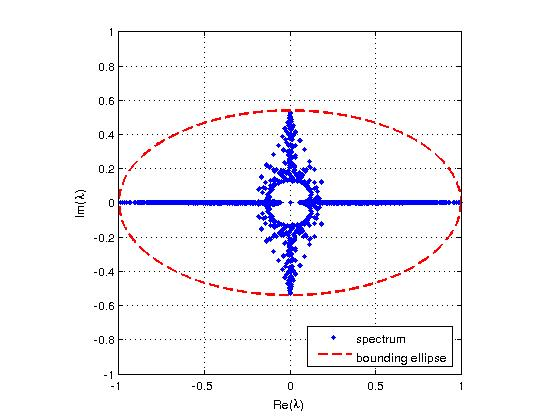
\includegraphics[width=\textwidth]
                    {spectrum0.jpg}
    \caption{0th order}
  \end{subfigure}
    \begin{subfigure}[b]{0.49\textwidth}
      \centering
      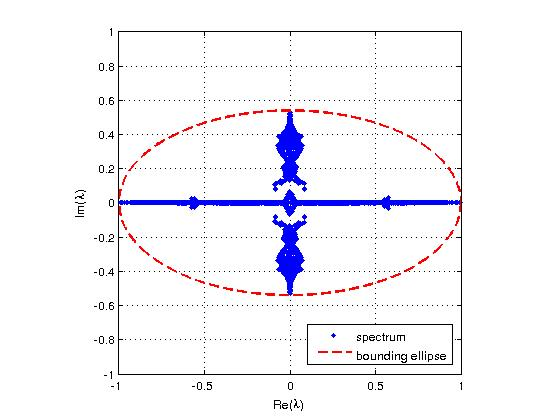
\includegraphics[width=\textwidth]
                      {spectrum2.jpg}
      \caption{2nd order}
    \end{subfigure}
    \caption{Representative current eigenspectra for the IAEA problem.  In both 
             cases the maximum modulus along the imaginary axis is 
             $\epsilon \approx 0.54$.}            
  \label{fig:spectrum}            
\end{figure}


Despite these theoretical limitations, recent work claims to have 
used Chebyshev acceleration successfully for solving the inner 
problem \cite{zhang2012ehs}.  However, it seems likely its success would 
be highly problem-dependent and subject to significant tuning, two 
features we would ultimately choose to avoid.


\subsubsection{Krylov Subspace Methods}

As an alternative to the power method, we investigate Krylov subspace 
methods for the eigenvalue problem, the most well-known of which is 
the Arnoldi method.  The Arnoldi method entails generation
of the Krylov subspace defined by Eq. \ref{eq:krylovsubspace}.
The Arnoldi process is used as in GMRES to obtain the 
upper Hessenberg matrix $\mathbf{H} \in \mathbb{R}^{n \times n}$. It turns 
out that the eigenvalues of $\oper{H}$, called ``Ritz values,'' tend to
be good estimates of eigenvalues of $\oper{A}$, and given an eigenpair
$(\tilde{\lambda}, y)$ of $\oper{H}_m$, the Rayleigh-Ritz estimate of the
corresponding eigenvector of $\oper{A}$ is defined $x = \oper{V}_m y$, 
and is called a ``Ritz vector.''

The eigenpairs of $\oper{H}$ are found via a dense eigensolver, such as 
the QR method.  While this is done on a small system (since $m \ll n$), 
it is done repeatedly for increasing $m$ until some criterion is met.  
If $m$ becomes too large, the dense methods become too expensive.  To 
circumvent this issue, the Arnoldi method must be restarted.  In 
the {\it explicitly} restarted Arnoldi method (ERAM), some combination of 
the existing $m$ Ritz vectors is used to choose a single starting guess, 
from which a new Arnoldi factorization is generated.  There are several ways 
to do this; in this work, the default SLEPc implementation is used, 
described in Ref. \cite{slepc-str-4}.

An alternative to explicit restart is {\it implicit} restart, where the 
desired portion of the spectrum is retained continuously by contracting 
from a subspace of dimension $m$ to a smaller space of size $p$ and mapping 
back to the larger space.  This is done via implicitly-shifted QR, and leads 
to the implicitly-restarted Arnoldi method (IRAM) \cite{sorensen1992iap}.  
An alternative to IRAM used in this work is the Krylov-Schur (KS) method
\cite{stewart2002ksa}, which transforms a general Krylov decomposition 
(of which the Arnoldi decomposition is a special case) into a Krylov-Schur 
decomposition,
where the upper Hessenberg matrix $\oper{H}$ above becomes a strictly upper
triangle matrix $\oper{T}$.  Using this decomposition, it is comparatively
easier numerically to keep the desired spectral information, and the method is
apparently often more efficient than IRAM.  As for ERAM, the default SLEPc
implementation of KS is used; the method and its implementation in SLEPc are
described in Ref. \cite{slepc-str-7}.

%----------------------------------------------------------------------------%
\subsection{Accelerating the Fixed Point Iteration}

In the sections to follow, we investigate several techniques for 
accelerating the outer fixed point iteration for $k$.  All 
the methods are based on some form of extrapolation with respect to 
$k$, and hence no machinery beyond that needed for the 
fixed point iteration is required for their use.

%----------------------------------------------------------------------------%
\subsubsection{Regula Falsi and Related Methods}
\label{sec:extrapolationmethods}

\index{regula falsi}

Recall that the current eigenvalue $\lambda$ approaches unity in the 
limit $k\to k^*$.  For conservative responses with negligible 
iteration error, $\lambda$ tends to {\it exactly} unity.  Various 
schemes have been used to capitalize on this relationship.  In each 
case, an initial guess $k_0$ is made for which the corresponding 
$\lambda_0$ is found.  Subsequently, $k_1$ is selected, potentially via 
balance, and $\lambda_1$ is computed.  All successive values $k_n$  
are selected so that $\lambda_n \approx 1$.  Such a scheme is often
called {\it regula falsi} or the {\it method of false points} 
\cite{lindahl1976mdr}.

% see page 71.  He explicitly states that 1/L~1/k is better than 1/L~k and
% L~k
Lindahl studied the relationship between $\lambda$ and $k$ and found that 
$\tilde{k} = 1/k$ varies quite 
linearly with $\tilde{\lambda} \propto 1/\lambda$.
Lindahl extended the concept by storing three or more pairs for interpolation
via higher order polynomials \cite{lindahl1976mdr}.

Anghel and Gheorghu \cite{anghel1987isr}
modified the approach of Lindahl by assuming the 
exponential relation
\begin{equation}
  \lambda \propto a e^{b/k} \, .
\end{equation}
Because response functions tend to have exponential dependence on 
$k$, they assumed that would also apply to the current eigenvalue.  As the
results below will indicate, this form compares favorably with Lindahl's.

A more recent study by Forget and Rahnema \cite{forget2005nee} 
rediscovered the relationship
between $k$ and $\lambda$, the latter of which they denoted
the ``normalization constant.'' 
Moving from a $k$-update via balance, they assumed the relation 
$k \propto 1/\lambda$ and found good results.  In theory, we might expect 
this to be the case.  Expanding the result of Eq. \ref{eq:dlambda_db_asy}
for small $B$, we find that 
\begin{equation}
 \frac{d \lambda}{d B} \propto  B \, ,
\end{equation}
suggesting that 
\begin{equation}
 \lambda \approx  a B^2 + b \approx \frac{a'}{k} + b' \, .
\end{equation}
Of course, this is based on a one group approximation in the limit of 
very small nodes. Interestingly, Lindahl
found that $k^{-1} \propto \lambda^{-1}$ produced better results, having 
compared to both $k \propto \lambda^{-1}$ and $k \propto \lambda$ (though
without giving numerical results) \cite{lindahl1976mdr}.

All four two-term schemes have been implemented and are assessed in 
the results to follow.  A key limitation of these schemes is that they 
depend on $\lambda$ getting to unity, or at least close enough so that
its departure from unity is within the convergence criteria used.  If
either the responses or the inner iterations are poorly converged, or
the response expansions are not conservative, the 
schemes can become unstable.


%----------------------------------------------------------------------------%
\subsubsection{Steffensen's Method}
\label{sec:steffensensmethod}

\index{Steffensen's method}
\index{Aitken's method}

A similar approach to those described above is Steffensen's method, which, 
like the others, relies on a sequence of evaluations of the fixed point.
Steffensen's method is most easily motivated via use of
Aitken's $\delta^2$ process. Consider a monotonic sequence
\begin{equation}
  \left \{k \right \} \equiv 
    \left \{ k_0, k_1, k_2, \ldots, k_n, \ldots \right \}
\end{equation}
such that
\begin{equation}
 \lim_{n\to \infty} k_n = k^* \, .
\end{equation}
If the sequence is linearly convergent, then
\begin{equation}
 \frac{k_{n-1} - k^*}{k_{n-2} - k^*} 
   \approx  \frac{k_{n} - k^*}{k_{n-1} - k^*} \, .
\end{equation}
Consequently, 
\begin{equation}
 (k_{n-1} - k^*)^2 \approx (k_{n} - k^*)(k_{n-2} - k^*) \,
\end{equation}
yielding Aitken's $\delta^2$ approximation
\begin{equation}
 k^* \approx k^*_{n} 
   = k_{n-2} - \frac{ (k_{n-1} - k_{n-2})^2 }
                    { k_{n} - 2 k_{n-1} + k_{n-2} } \, .
\end{equation}

Suppose the sequence is generated by a series of Picard
iterations as defined in Eq. \ref{eq:picard}.
If the improved estimate $k^*_{n}$ is used in place of $k_n$, the 
resulting iteration is referred to as Steffensen's method.  Since 
this is akin to extrapolation by a second order polynomial fit, we might 
expect the improved estimate yields an iterative scheme 
of second order, which is indeed true for Steffensen's method.

Steffensen's method can be written as the one step fixed point iteration
\begin{equation}
 k' = g(k) = k - \frac{(f(k) - k)^2} 
                     {f(f(k)) - 2 f(k) + k}  \, .
\end{equation}
Following Section \ref{sec:fixedpointiteration}, we expand $g(k)$ about
the fixed point $k^*$, yielding 
\begin{equation}
 g(k) = g(k^*) + \Delta g'(k^*) + \frac{\Delta^2}{2} g''(k^*) 
               + \mathcal{O}(\Delta^3) \, .
\end{equation}
To be (at least) second order, $g'(k^*)$ must vanish.  Here,
\begin{equation}
\begin{split}
  \lim_{k\to k^*}
    g'(k) &= 1 - \frac{2(k-f(k))(1-f'(k))}
                      {f(f(k))-2f(k)+k}\\
          & \quad + \frac{(k-f(k))^2(f'(f(k))f'(k) - 2f'(k)+1)}
                      {(f(f(k))-2f(k)+k)^2} \\
          &= 1 - (2) + (1) \\
          &= 0 \, ,
\end{split}
\end{equation}
where the second two terms are reduced via L'H\^{o}pital's rule.

In practice, Steffensen's method is highly sensitive to the 
accuracy of the sequence estimates.  Within the ERMM, it
has been observed that Steffensen's method becomes unstable
unless very small tolerances ($\approx 10^{-9}$) are used 
for solving the $\lambda$-eigenvalue problem.

Furthermore, note that once the responses are evaluated for the initial
guess, each successive Steffensen iteration requires two response 
evaluations.  In general, the savings gained by second order convergence 
may or may not outweigh the cost of additional evaluations depending 
on the problem.


%----------------------------------------------------------------------------%
\subsection{Solving ERME's via Newton's Method}
\label{sec:newtonsmethod}

\index{Newton's method}

The eigenvalue response matrix problem has been recognized as a 
nonlinear problem since it was first solved, but it does not 
appear it has been cast in a form for solution directly by 
Newton-based methods until quite recently \cite{roberts2010ncm}.  

\index{nonlinear residual of ERME}

The eigenvalue response matrix equation, $k$ update equation, 
and $L_2$ normalization of $J_{-}$ can be written as the nonlinear 
residual
    \begin{equation}
    \mathbf{f(x)} = \left [\begin{array}{c}
            (\mathbf{M}\mathbf{R}(k)-\lambda \mathbf{I}) \mathbf{J_-} \\
            \mathbf{F}(k)\mathbf{J_-} - (k\mathbf{L}(k)\mathbf{J_-} ) \\
            \frac{1}{2} \mathbf{J^T_-} \mathbf{J_-} - \frac{1}{2}  
          \end{array} 
    \right ]  = \mathbf{0} \, ,
    \label{eq:residual}
    \end{equation}
and the associated \index{Jacobian of ERME} Jacobian is defined
  \begin{equation}
  \mathbf{f'(x)} = \left [\begin{array}{ccc}
          (\mathbf{M}\mathbf{R}-\lambda \mathbf{I})  
          &  \mathbf{M}\mathbf{R_k}\mathbf{J_-}                     
          & \mathbf{J_-}  \\
          (\mathbf{F}-k\mathbf{L})                   
          &  (\mathbf{F_k}-k\mathbf{L_k}-\mathbf{L}) \mathbf{J_-}   
          & 0  \\
          \mathbf{J^T_-}                             
          & 0                                                       
          & 0
        \end{array} 
  \right ]  \, .
  \label{eq:jacobian}
  \end{equation}
For $\mathbf{R}(k)$ of size $m\times m$, the Jacobian is of 
size $(m+2)\times(m+2)$.  Moreover, after one evaluation of 
the response quantities, only the first $m+1$ rows of the $(m+1)$th 
column of $\mathbf{f'}$ are not known {\it a priori}, and that 
unknown column requires only one additional evaluation of the 
response quantities to allow for a finite difference 
approximation of the partial derivatives with respect to $k$.
Hence, like Steffensen's method, Newton's method requires two 
evaluations of $k$ per iteration, if the latter approximates the 
derivative via functions evaluated at $k$ and $k + \delta k$.  
Typically, a value of 
$\delta k \approx \sqrt{\epsilon_{\text{machine}}} \approx 10^{-8}$
is close to optimal.  However, at likely reduced performance, the 
finite difference can make use of previous values of $k$;  in this 
case, convergence would likely improve every iteration as each $k$ 
is closer to the solution.  
% Both schemes are tested in the next 
% chapter, and for the most part, the slight reduction in the 
% derivative accuracy and its effect on convergence is far outweighed 
% by the savings due to reducing the number of $k$ evaluations required.

%----------------------------------------------------------------------------%
\subsubsection{Newton's Method}

Newton's method \cite{kelley1995iml} solves a nonlinear system 
via the sequence
\begin{equation}
 \mathbf{s} = -\mathbf{f}'(\mathbf{x}^{(n)})^{-1} \mathbf{f}(\mathbf{x}^{(n)})
 \label{eq:newtonstep}
\end{equation}
where $\mathbf{s}$ is the Newton step, and the Newton update is
\begin{equation}
 \mathbf{x}^{(n+1)} = \mathbf{x}^{(n)} + l \mathbf{s} \, ,
 \label{eq:newtonupdate}
\end{equation}
with a step length $l$ defined to guarantee a decrease in 
$||\mathbf{f(x)}||_2$.  If a solution $\mathbf{x}^*$ exists, 
and $\mathbf{f}'$ is Lipschitz continuous near and nonsingular 
at $\mathbf{x}^*$, then Newton's method is known to exhibit 
quadratic convergence \cite{kelley1995iml}.  

For the nonlinear residual of Eq. \ref{eq:residual} and 
Jacobian of Eq. \ref{eq:jacobian}, these constraints appear to 
be true in practice.  For a standard, non-parameterized eigenvalue 
problem $Ax = \lambda x$, Peters and Wilkinson \cite{peters1979iii} 
have shown the associated Jacobian (akin to Eq. \ref{eq:jacobian} 
without the the $(m+1)$th column and row) is nonsingular at the 
solution if $\lambda$ is simple (which is true for the dominant 
mode of interest \cite{lindahl1981rrm}); however, it does not 
appear this is always true for the full Jacobian in 
Eq. \ref{eq:jacobian}, though in practice the conditions for 
singularity have not been encountered.

%----------------------------------------------------------------------------%
\subsubsection{Inexact Newton and JFNK}

\index{inexact Newton methods}
\index{Jacobian-free Newton-Krylov}

An inexact Newton method uses an approximate linear solve for 
the Newton step satisfying 
\begin{equation}
 || \mathbf{f}'({x}^{(n)}) \mathbf{s} + \mathbf{f}(\mathbf{x}^{(n)}) ||_2  
   \le \eta || \mathbf{x}^{(n)} ||_2 \, ,
 \label{eq:inexactnewtonstep}
\end{equation}
where $\eta$ is the ``forcing term'' that may vary at each 
iteration \cite{kelley1995iml}. 
The inexact solution of the Newton step necessarily 
impacts convergence of Newton's method, but typically convergence 
remains superlinear.  In general, any iterative method for a linear 
system could be used, but we focus on the specific application of 
Krylov solvers, yielding Newton-Krylov methods.

Since solving for $\mathbf{s}$ involves only the action of the 
Jacobian, the Jacobian need not be explicitly formed.  Then 
Newton-Krylov methods become  Jacobian-Free Newton-Krylov (JFNK) 
methods, for which Knoll and Keyes provide an extensive survey 
\cite{knoll2004jfn}.  If the action of $\mathbf{MR}$ were performed 
in a matrix-free 
manner, the same algorithm could be used in evaluating the 
action of $\mathbf{f}'$ for a fully matrix-free approach.

Often in the context of JFNK, the action 
of the Jacobian is approximated as a finite difference 
approximation; however, since the Jacobian in Eq. \ref{eq:jacobian} 
is defined almost entirely {\it a priori}, only a relatively small 
portion of the action need be approximated via finite differences.  
This is critical for on-the-fly response generation, for which
evaluation of $k$-dependent responses is the dominant cost, since
each Krylov vector generally represents a perturbed $k$.

%----------------------------------------------------------------------------%
\subsubsection{Preconditioning JFNK}

The key to effective use of Krylov-based linear solvers is often 
adequate preconditioning.  For JFNK, a preconditioner $\mathbf{M}$ is 
in some way ``close'' to the Jacobian $\mathbf{f}'$ but is easier to 
construct or apply.  Moreover, $\mathbf{M}$ can be applied either 
to the left, yielding the 
system $\mathbf{M}^{-1}\mathbf{f}'\mathbf{s}=-\mathbf{M}^{-1}\mathbf{f}$, or 
to the right by solving 
$\mathbf{f}' \mathbf{M}^{-1} \tilde{\mathbf{s}} = -\mathbf{f}$ and 
setting $\mathbf{s} =  \mathbf{M}^{-1} \tilde{\mathbf{s}} $.

In the numerical studies of the next chapter, we employ incomplete 
factorization using an approximate Jacobian matrix as a basis.  
The easiest choice is to use a full Jacobian computed using the 
initial guess (which itself has been preconditioned by a single 
coarse Picard iteration), possibly omitting the partial derivatives 
to save on a function evaluation.  While this approximate Jacobian 
requires the explicit construction of $\mathbf{MR}$, this is 
relatively easy to do given the extreme sparsity of $\mathbf{M}$.


%-------------------------------*- Mode:TeX -*-------------------------------%
\section{Comparison of ERME Solvers}
\label{sec:erme_solver_results}


In this chapter, the solvers developed in 
Chapter \ref{sec:newton} are applied to several benchmark
problems.  The purpose is largely two-fold.  While previous chapters 
have discussed in some depth the accuracy of various approximations,
a further comparison based on somewhat larger, more representative 
problems is valuable.  Secondly, and more importantly, we aim to 
assess which of the various algorithms is best suited for solving 
response matrix equations.

\subsection{Diffusion Benchmarks}

Several diffusion benchmarks were first used to investigate the 
various response matrix algorithms previously described.  While 
such benchmarks do not represent particularly 
``challenging'' problems by modern 
standards, they are simple to model and provide easy 
application problems for testing the solvers (and expansions schemes)
to a fully converged state.

The problems considered are the 2-D and 3-D IAEA benchmarks, and the 
2-D Biblis problem, all two-group problems, and the four-group, 2-D 
Koeberg benchmark.  Each problem is based on homogenized assemblies, 
and brief specifications are provided in Appendix \ref{app:benchmarks}.

For all problems, the multigroup dependence is exactly treated while the 
spatial dependence is expanded in DLPs.  Each 2-D assembly is discretized 
using a $20\times 20$ spatial mesh, corresponding roughly to 1 cm square 
cells.  For the 3-D IAEA problem, 20 cm cubes are represented by a
$10 \times 10 \times 10$ spatial mesh to reduce the size of the 
reference calculation.
While the discretizations used are not 
  fully spatially-converged grids, they are adequate 
 for the present study.  The reference solution uses the same 
mesh spacing for consistency.  

When computing responses, no symmetry is considered.  For homogeneous
problems, exploiting symmetry would reduce the number of responses 
by a factor of 4 in 2-D or a factor of 6 in 3-D.  Such tricks are 
of course handy for benchmarking, but in reality, reactor assemblies 
are only symmetric at beginning-of-life (and that is on the order 
of 1/3 of the core fuel), and even then, only at cold zero power.  Once
any realistic treatment of temperature feedback is considered, all 
symmetry is lost, and hence there is essentially no insight to be gained 
from artificially reducing our problem size.

Unless stated otherwise, 
convergence is defined by $||\oper{f}||_2 \leq 10^{-7}$, where
$\oper{f}$ is the nonlinear residual defined by Eq. \ref{eq:residual}.
Using this criterion makes comparison of Picard and Newton methods much 
more straightforward.  The reference fine mesh solution uses a tolerance 
of $10^{-12}$, though this applies to the 
residual $\oper{A}\phi-\lambda \phi$ of the fine mesh eigenvalue problem.

\subsubsection{Tolerances and Errors}

As was discovered in early chapters, a convergence criterion based on 
one quantity may not be an accurate measure of the error in some 
other quantity.  To illustrate, the assembly powers for the 2-D IAEA 
problem were computed for spatial orders of 0 through 4 subject to 
a tolerance on the residual norm ranging from $10^{-1}$ down to $10^{-12}$.
The relative eigenvalue error for each order as a function of 
tolerance is shown in Figure \ref{fig:tolerance_study_eigenvalue}, 
while the 
maximum relative assembly error for each order is shown in 
Figure \ref{fig:tolerance_study_power}.  The latter figure
indicates that the {\it convergence} error in assembly powers 
for a  given order is vanishingly small compared to 
the {\it truncation} error due to the order for tolerances
below about $10^{-6}$.  A similar trend appears for the eigenvalue 
error, but for even looser tolerances.  For the subsequent diffusion 
analyses, a tolerance of $10^{-7}$ was selected to ensure only 
truncation errors affect the solutions observed.

\begin{figure}[ht]
    \centering
    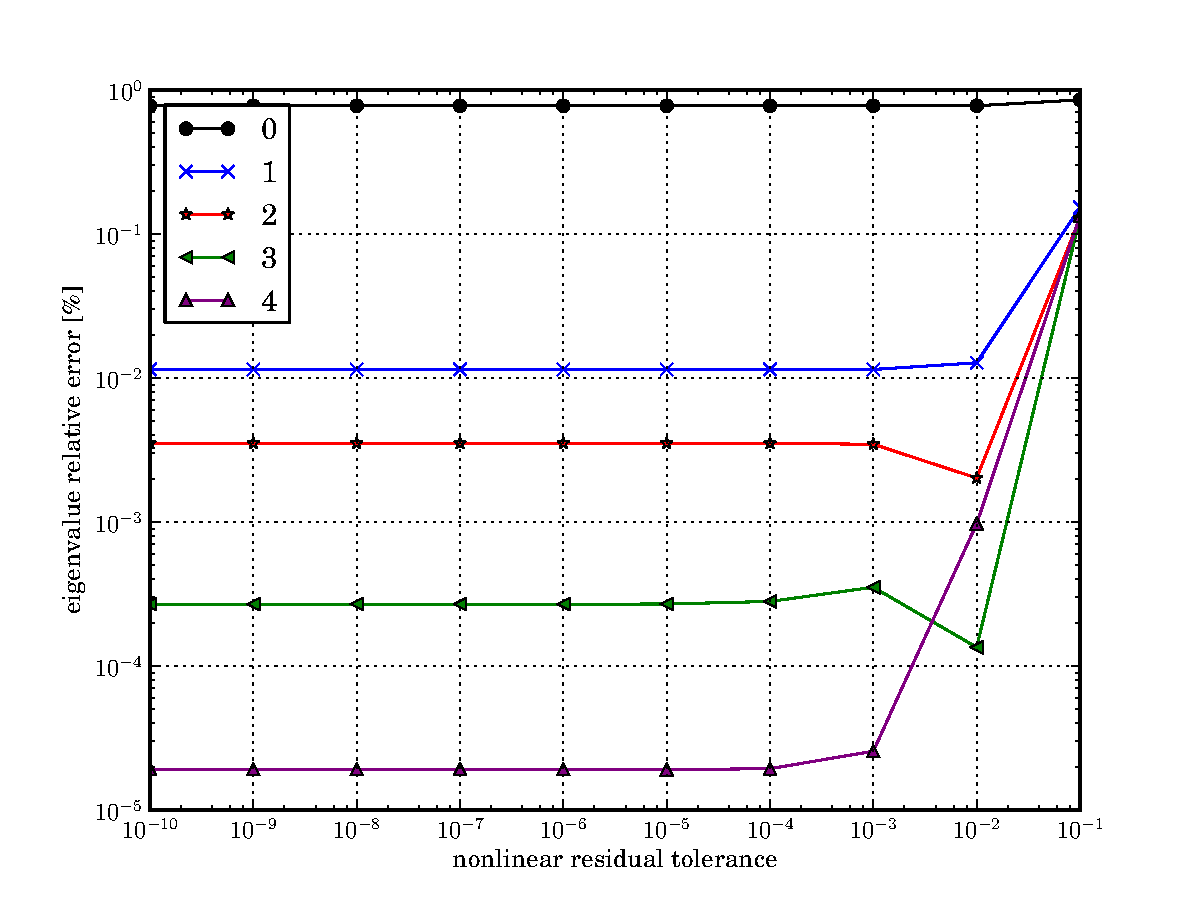
\includegraphics[keepaspectratio, width = 5.0 in]
                    {tolerance_study_eigenvalue}
    \caption{Absolute relative eigenvalue error for the 2-D IAEA 
             problem as a function of residual 
             norm tolerance for several spatial orders .}
    \label{fig:tolerance_study_eigenvalue}
\end{figure}

\begin{figure}[ht]
    \centering
    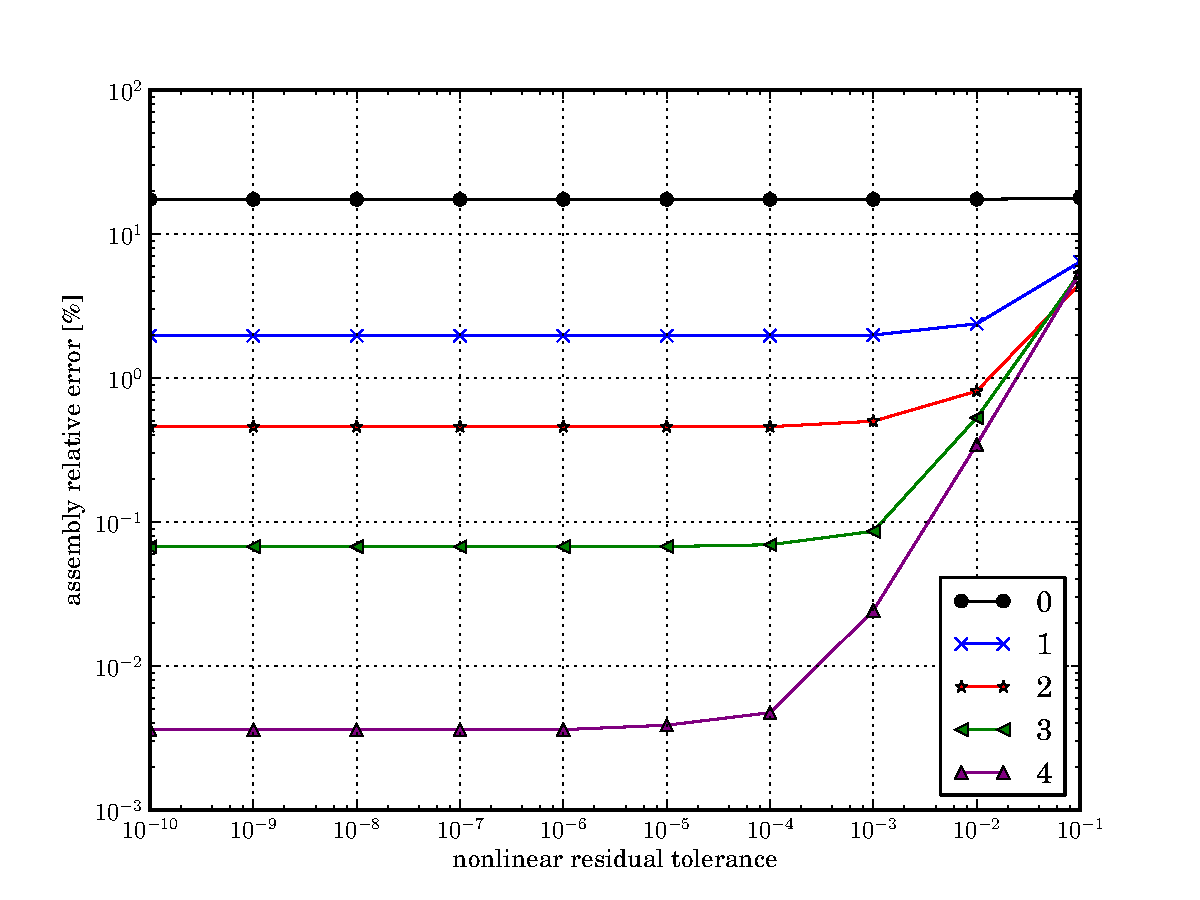
\includegraphics[keepaspectratio, width = 5.0 in]
                    {tolerance_study_power}
    \caption{Maximum absolute relative assembly power error for the 2-D IAEA 
             problem as a function of 
             residual norm tolerance for several spatial orders.}
    \label{fig:tolerance_study_power}
\end{figure}

\subsubsection{Orders and Accuracy}
\label{sec:diffusion_order_accuracy}

While some attention was paid to the accuracy of spatial expansions in 
Chapter \ref{sec:expansion}, it is illustrative to assess convergence 
of the DLP basis applied to the diffusion benchmarks.  
Figure \ref{fig:diffusion_order_study_power}
 shows the maximum relative error in the assembly 
powers as a function of spatial order, while Figure 
\ref{fig:diffusion_order_study_eigenvalue} does 
the same for the absolute relative error in the eigenvalue.  For the 
3-D IAEA problem, two cases are performed.  The first uses a full 
expansion of order $m$ in both spatial variables.  That means on a given 
side, the two-dimensional expansion is equivalent to the form 
\begin{equation}
 F(x, y) \approx a + bx + cy + d x^2 + e xy + f y^2 + \ldots \, .
\end{equation}
The second case uses an order reduction scheme that 
limits the sum of the $x$ and $y$ orders \cite{forget2006tdh}.  In this case,
\begin{equation}
 F(x, y) \approx a + bx + cy + d x^2 + f y^2 + \ldots \, ,
\end{equation}
where the cross term $e xy$ has been omitted.  Previous experience 
has demonstrated these cross terms, particularly at high order, have 
little value, and this is demonstrated quite strongly in the results
of Figures \ref{fig:diffusion_order_study_eigenvalue} 
and \ref{fig:diffusion_order_study_power}.

% Say something about the reduction in unknowns, the total node count, 
% etc.

For all the problems, a fourth order expansion yields assembly 
(or nodal, for the IAEA-3D problem) errors below a tenth of a percent 
and eigenvalue errors on the range of a few pcm.  Consequently, a fourth 
order expansion was selected for use in comparing the solvers in 
subsequent performance analyses.

\begin{figure}[ht]
    \centering
    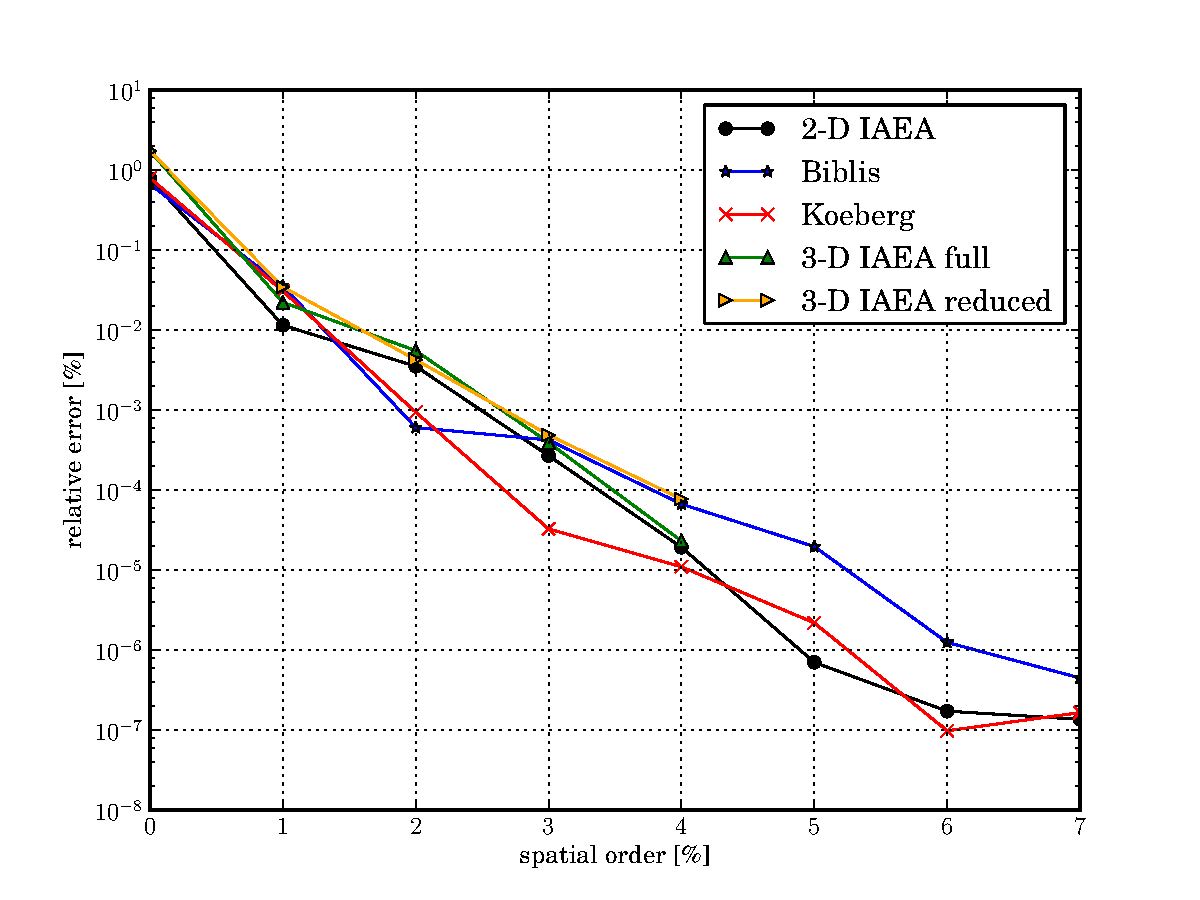
\includegraphics[keepaspectratio, width = 5.0 in]
                    {diffusion_order_study_eigenvalue}
    \caption{Absolute relative eigenvalue error as 
             a function of spatial order.}
    \label{fig:diffusion_order_study_eigenvalue}
\end{figure}

\begin{figure}[ht]
    \centering
    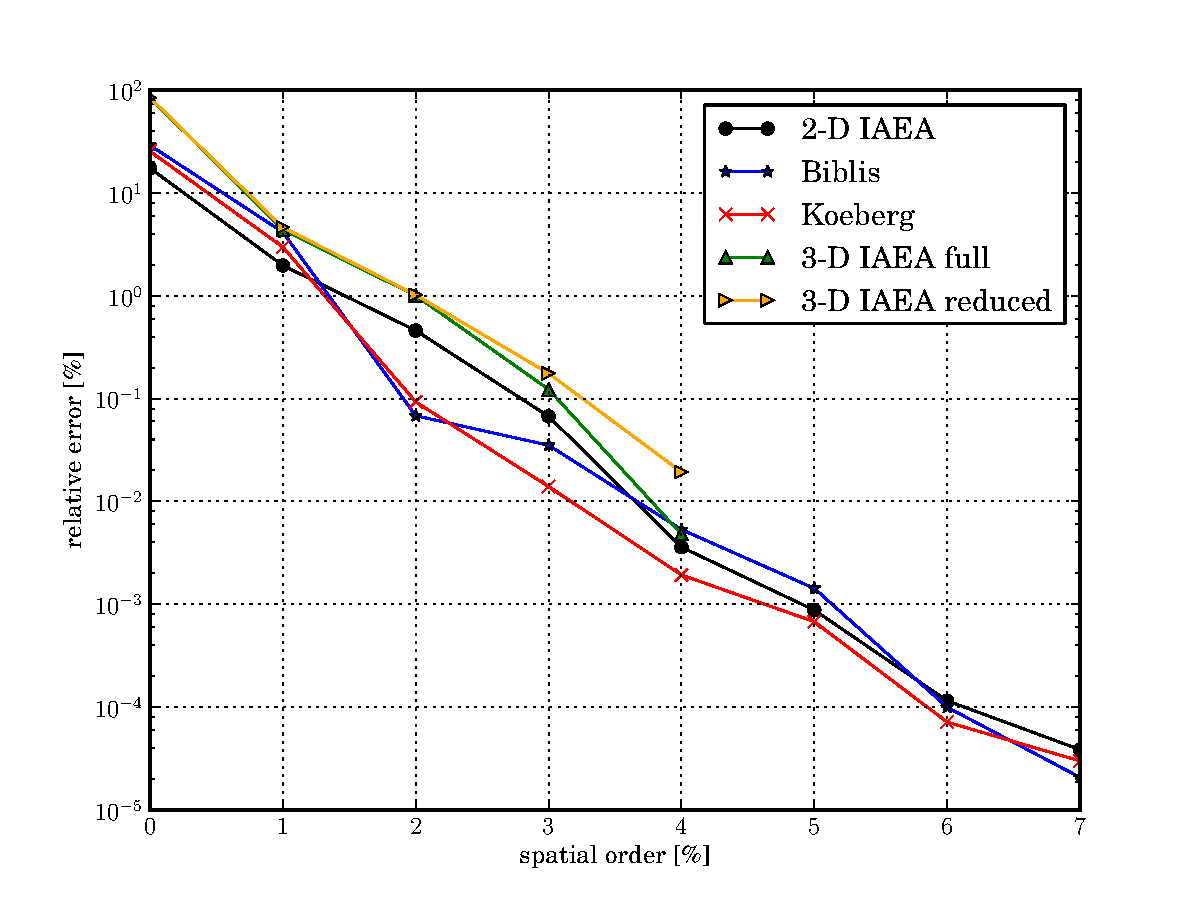
\includegraphics[keepaspectratio, width = 5.0 in]
                    {diffusion_order_study_power}
    \caption{Maximum absolute relative assembly power error as a function of 
             spatial order.}
    \label{fig:diffusion_order_study_power}
\end{figure}

\subsubsection{Inner Solver Comparison}

For use in the Picard solver, several eigenvalue solvers were investigated 
to solve the inner $\lambda$-eigenvalue problem, including the 
power (PI), Krylov-Schur (KS), and explicitly-restarted Arnoldi 
methods (ERAM), each of 
which is implemented in SLEPc \cite{slepc}.  Because convergence of the 
outer Picard iteration is somewhat sensitive to the inner convergence, 
the tolerance $\tau_{\lambda}$ of the inner problem was set 
more tightly at $10^{-10}$.  

Table \ref{tbl:diffusion_picard_inner_study} 
provides the number of inner and outer iterations and total
computational time for each method for each of the diffusion problems.
The computational time is further divided into the global (response matrix)
time and the response (diffusion solver) time.  For all problems, 
KS outperforms ERAM by a small margin and PI by a factor of two 
or three.  Initial studies demonstrated that IRAM (not included 
by default with SLEPc) performs at about the same level 
as KS \cite{roberts2012ksi}. Were the tolerance smaller, the improvement 
of KS over PI would 
likely diminish, and were the tolerance greater, KS would likely perform 
increasingly better.  

For the three 2-D problems, the response time constitutes a significant 
portion of the total computational time, range from about a third to half
depending on the solver.  For the 3-D IAEA problem, the global solver
becomes the dominant cost.  This makes some sense, as the diffusion 
problems underlying the response generation are quite cheap compared to 
the much larger global problem.

\begin{table}[ht] 
 \begin{center} 
 
 \begin{threeparttable}

 
 \begin{tabular}{ccccc} 
 \toprule 
  solver & time [s] & r. time [s]\tnote{a} & inners & outers \\
 \midrule 
              &  \multicolumn{4}{c}{2-D IAEA} \\ 
 \midrule 
           PI &      1.87 &      0.37 &         3416 &            6 \\ 
           KS &      0.69 &      0.41 &           33 &            6 \\ 
         ERAM &      0.77 &      0.40 &           36 &            6 \\ 
 \midrule 
              &  \multicolumn{4}{c}{Biblis} \\ 
 \midrule 
           PI &      2.16 &      0.68 &         3437 &            5 \\ 
           KS &      0.97 &      0.68 &           31 &            5 \\ 
         ERAM &      1.05 &      0.69 &           34 &            5 \\ 
 \midrule 
              &  \multicolumn{4}{c}{Koeberg} \\ 
 \midrule 
           PI &      5.83 &      1.62 &         2012 &            3 \\ 
           KS &      2.38 &      1.66 &           21 &            3 \\ 
         ERAM &      2.63 &      1.67 &           21 &            3 \\ 
 \midrule 
              &  \multicolumn{4}{c}{3-D IAEA} \\ 
 \midrule 
           PI &    910.63 &     18.77 &         4427 &            6 \\ 
           KS &    210.91 &     19.47 &           75 &            6 \\ 
         ERAM &    294.48 &     19.75 &           70 &            6 \\ 
 \bottomrule 
 \end{tabular} 
 

 {\footnotesize
 \begin{tablenotes}
   \item[a] Response generation time
 \end{tablenotes}
 }
 \end{threeparttable}
 
 
 
 \end{center} 
 \caption{Picard inner solver comparison for diffusion problems.} 
 \label{tbl:diffusion_picard_inner_study} 
\end{table} 


\subsubsection{Outer Solver Comparison}

Because KS was the best of the inner solvers investigated, it was 
selected for studies of the Picard-based outer iteration schemes.
For this study, Picard iteration along with the accelerated variant 
based on the {\it regula falsi} method was compared to Steffensen's 
method and Newton's method.  

\subsubsection{Picard Acceleration}

The four Picard acceleration schemes were applied to the 2-D IAEA 
and Koeberg problems
using a fourth order expansion.  
Figure \ref{fig:diffusion_picard_acceleration}
shows the nonlinear residual as a function of outer iteration for the 
unaccelerated case along with the four accelerated cases. 

As the numerical results of the last section and of Chapter 
\ref{sec:fixedpoint} show, the Picard iteration by itself is a 
quickly converging process.  However, the acceleration schemes
can offer some improvement.  Here,
 exponential and inverse-inverse extrapolation provide the 
most robust improvement, though they actually provide no reduction 
in iterations for the Koeberg problem.
Recall that all the schemes depend critically
on the limit $\lambda \to 1$, and this only occurs if the responses are 
computed very accurately and the responses are conservative.  Here, the 
 diffusion responses are computed essentially by LU factorization since 
 they are such small problems and are conservative based on the 
 uniform mesh and DLP expansion.  Even so, the linear-inverse and 
 linear-linear suffer from their sensitivity to round-off errors, and
 while care was taken when implementing the coefficients, the convergence 
 tolerances used are apparently not tight enough to ensure stability.
Because the exponential scheme yields a slightly smaller final residual
norm, it was included for study with the remaining algorithms.
 
\begin{figure}[ht]
    \centering
    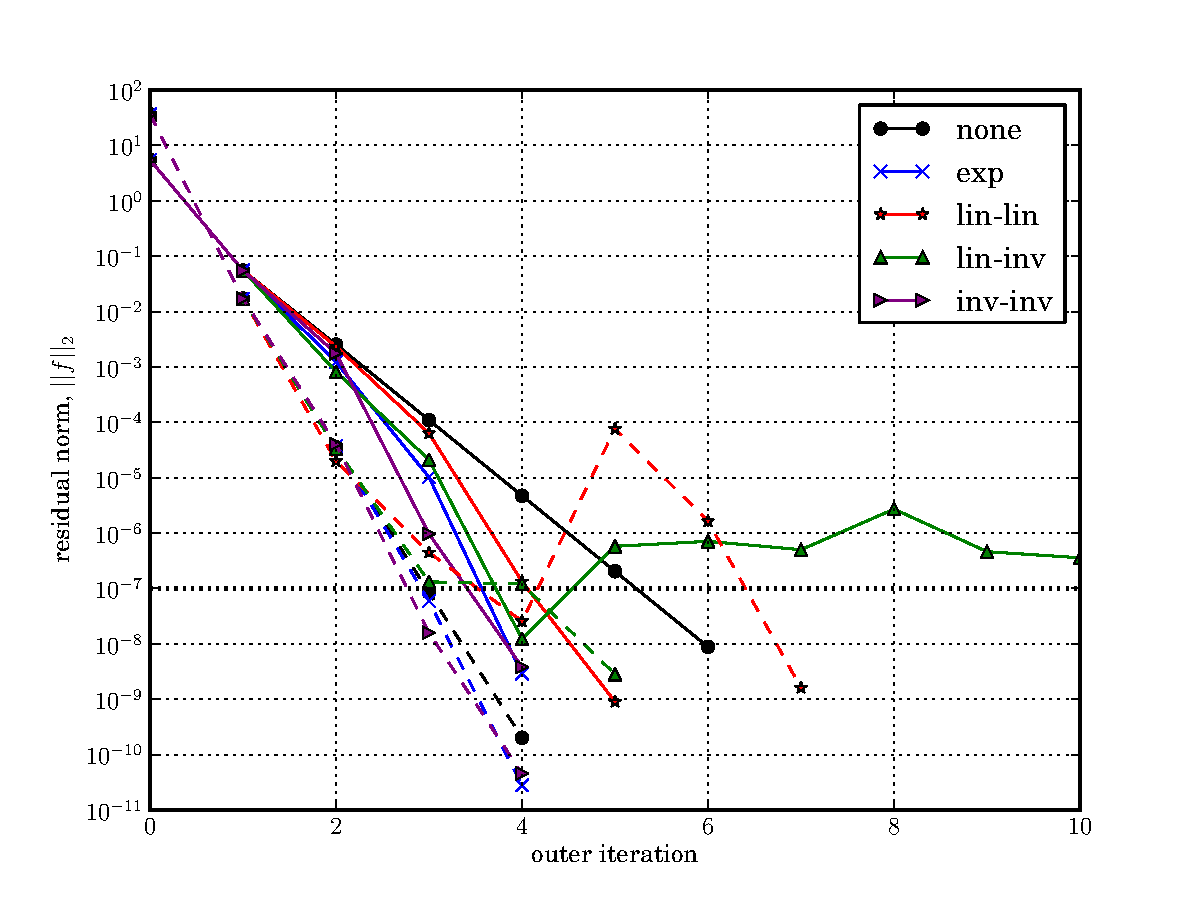
\includegraphics[keepaspectratio, width = 5.0 in]
                    {diffusion_picard_acceleration}
    \caption{Comparison of Picard acceleration schemes for the 
             2-D IAEA problem (solid lines) and Koeberg 
             problem (dashed lines).  }
    \label{fig:diffusion_picard_acceleration}
\end{figure}

\subsubsection{Newton Variants}

For Newton's method, both an unpreconditioned 
and ILU-preconditioned variant were studied.  The ILU preconditioner 
is based on an explicit Jacobian constructed either once, using the 
initial responses, or every iteration, using the updated responses.  
In all cases, the underlying linear solves were performed with GMRES(30),
and the ILU preconditioner was applied with 0 through 2 levels.

Table \ref{tbl:diffusion_newton_pc_study} provides results for the 
2-D IAEA and Koeberg problems using a fourth order spatial 
expansion and $4\times 4$ nodes per assembly.  This yields a 
somewhat larger problem that better illustrates differences 
in the preconditioner; the preconditioners offer no benefit 
for the single node case.  The problems have 184962 and 
369922 unknowns, respectively.

For both problems, ILU(0) preconditioning offers the best performance
with respect to time despite higher levels yielding lower numbers of 
inner iterations.
Interestingly, not updating the preconditioner has no discernible effect 
on the iteration count and yields lower computational times than when 
the preconditioner is updated at every iteration.  This can be explained 
by noting that the majority of the Jacobian is relatively insensitive 
to small changes in $k$.  Given the initial guess (unity in these cases)
is expected to be pretty close to the final answer, the original Jacobian
should be pretty close to its final value.


\begin{table}[ht] 
 \begin{center} 
 
 \begin{threeparttable}

 \begin{tabular}{ccccc} 
 \toprule 
  preconditioner & time [s] & r. time [s]\tnote{a} & inners & outers \\
 \midrule 
 &  \multicolumn{4}{c}{2-D IAEA} \\ 
 \midrule 
          none &     12.62 &      0.46 &          477 &            4 \\ 
  no update ILU(0) &     10.43 &      0.46 &          144 &            4 \\ 
  no update ILU(1) &     11.68 &      0.46 &          118 &            4 \\ 
  no update ILU(2) &     12.37 &      0.46 &           86 &            4 \\ 
        ILU(0) &     10.69 &      0.46 &          144 &            4 \\ 
        ILU(1) &     14.07 &      0.45 &          118 &            4 \\ 
        ILU(2) &     17.12 &      0.45 &           86 &            4 \\ 
 \midrule 
 &  \multicolumn{4}{c}{Koeberg} \\ 
 \midrule 
          none &     45.82 &      3.29 &          403 &            4 \\ 
  no update ILU(0) &     43.18 &      3.34 &          157 &            4 \\ 
  no update ILU(1) &     52.18 &      3.35 &          136 &            4 \\ 
  no update ILU(2) &     58.26 &      3.35 &           91 &            4 \\ 
        ILU(0) &     45.61 &      3.35 &          157 &            4 \\ 
        ILU(1) &     67.44 &      3.38 &          136 &            4 \\ 
        ILU(2) &     89.90 &      3.35 &           91 &            4 \\ 
 \bottomrule 
 \end{tabular} 
 

 {\footnotesize
 \begin{tablenotes}
   \item[a] Response generation time
 \end{tablenotes}
 }
 \end{threeparttable}
 
 
 \end{center} 
 \caption{Newton solver ILU preconditioner comparison for diffusion 
          problems.} 
 \label{tbl:diffusion_newton_pc_study} 
\end{table} 

\subsubsection{Comparing Picard, Steffensen, and Newton}
\label{sec:global_solver_diffusion}

To compare the methods, several metrics are of interest.  Ultimately, the 
wall clock time is of most importance.  However, the number of iterations 
of each method, both outer and inner, is also indicative of the 
algorithm performance independent of any particular implementation.
These data are provided in Table \ref{tbl:diffusion_outer_study} 
for each of the benchmarks. A fourth
order spatial expansion  was used throughout, with order reduction being 
applied to the 3-D IAEA problem.  For the 2-D problems, a $4\times 4$ 
node-per-assembly model is used, while for the 3-D IAEA problem,  
a single node is used.  This corresponds to 184962 unknowns for the 
2-D IAEA and Biblis problems, 369922 for the Koeberg problem, 
and 988382 for the 3-D IAEA problem.

\begin{table}[!] 

 \begin{center} 
 
 \begin{threeparttable}
 \begin{tabular}{cccccc} 
 \toprule 
  solver & time [s] & r. time [s]\tnote{f} & inners & outers & $k$-evaluations \\
 \midrule 
 &  \multicolumn{5}{c}{2-D IAEA} \\ 
 \midrule 
    P\tnote{a}        &     10.26 &      0.32 &           76 &            5 &            6 \\ 
    P+exp\tnote{b} &      9.09 &      0.27 &           65 &            4 &            5 \\ 
    S\tnote{c} &     11.20 &      0.39 &           80 &            3 &            7 \\ 
  N+$\delta k$\tnote{d} &     10.35 &      0.44 &          144 &            4 &            8 \\ 
  N+$\Delta k$\tnote{e} &     10.22 &      0.28 &          146 &            4 &            5 \\ 
 \midrule 
 &  \multicolumn{5}{c}{Koeberg} \\ 
 \midrule 
        P &      9.26 &      0.56 &           64 &            4 &            5 \\ 
    P+exp &      9.06 &      0.56 &           62 &            4 &            5 \\ 
    S &      9.36 &      0.56 &           64 &            2 &            5 \\ 
  N+$\delta k$ &     10.89 &      0.92 &          140 &            4 &            8 \\ 
  N+$\Delta k$ &     10.49 &      0.57 &          140 &            4 &            5 \\ 
 \midrule 
 &  \multicolumn{5}{c}{Biblis} \\ 
 \midrule 
    P &     25.65 &      1.61 &           54 &            3 &            4 \\ 
    P+exp &     25.76 &      1.62 &           54 &            3 &            4 \\ 
    S &     29.61 &      2.02 &           60 &            2 &            5 \\ 
  N+$\delta k$ &     43.10 &      3.26 &          157 &            4 &            8 \\ 
  N+$\Delta k$ &     42.07 &      2.05 &          157 &            4 &            5 \\ 
 \midrule 
 &  \multicolumn{5}{c}{3-D IAEA} \\ 
 \midrule 
        P &    213.51 &     17.93 &           75 &            6 &            7 \\ 
    P+exp &    167.93 &     12.79 &           62 &            4 &            5 \\ 
    S &    214.07 &     17.98 &           75 &            3 &            7 \\ 
  N+$\delta k$ &    269.36 &     20.93 &          129 &            4 &            8 \\ 
  N+$\Delta k$ &    261.27 &     13.02 &          129 &            4 &            5 \\ 
 \bottomrule 
 \end{tabular} 

 {\footnotesize
 \begin{tablenotes}
   \item[a] Picard 
   \item[b] Picard with exponential extrapolation
   \item[c] Steffensen
   \item[d] Newton with fine $k$ difference
   \item[e] Newton with coarse $k$ difference
   \item[f] Response generation time
 \end{tablenotes}
 }
 \end{threeparttable}
 
 \end{center} 
 
 \caption{Outer solver comparison for diffusion problems.} 
 \label{tbl:diffusion_outer_study} 
 
\end{table} 

%  \footnote{fine finite difference for $k$}
%  \footnote{coarse finite difference for $k$}

The solvers tested included Picard (P) with and without exponential 
extrapolation (exp), Steffensen's method (S), and Newton's method (N).
For Newton's method, two schemes were examined.  The first is the same 
as used for testing the preconditioning and is based on a Jacobian with 
$k$-derivatives computed using a finite difference 
with a $\Delta k = 10^{-8}$.
The second scheme 
lags the $k$ evaluation, using the last iterate 
for computing $\Delta k$.  This results in a larger $\Delta k$ and hence 
less accurate finite difference.  However, the accuracy of the finite 
difference has no observable effect on the convergence, 
and for all four problems,
the lagged approach has the same number of outer iterations as the 
regular approach but reduces the number of $k$ evaluations by nearly half.

Steffensen's method provides the fastest convergence with respect to 
outer iterations, but it relies on two $k$-evaluations per outer iteration.
Picard with exponential extrapolation yields the lowest computational 
time and the fewest $k$-evaluations.  While Newton's method with a 
coarse $\Delta k$ is competitive with respect to $k$-evaluations, the 
overhead of solving the linear systems is higher than the cost of the 
$\lambda$-eigenvalue problem in the Picard iteration.

% FIGURE

\subsubsection{Comments}

From the diffusion analyses, it appears that Picard iteration using 
KS for the inners and the exponential extrapolation for accelerating 
the outers yields the best performance.  The Newton methods perform 
about as well with respect to $k$-evaluations, but the cost of 
applying the method is higher per iteration than the Picard variants,
implying further work on preconditioning the inner solves is warranted.

\subsection{2-D C5G7}


The 2-D C5G7 transport benchmark is a small quarter core 
model consisting of two UO$_2$ assemblies and two MOX
assemblies, all surrounded by an assembly-width reflector.
The problem is specified in Appendix \ref{app:benchmarks}.  Additionally,
the transport approximations used are described, and 
the \Detran reference results used in the following analysis are compared 
to the MCNP reference results from the original specification.  
 
\subsubsection{Orders and Accuracy}
 
To assess the accuracy of the response schemes available for transport 
problems, the C5G7 benchmark was solved using both a DLP and 
Chebyshev-Legendre basis in angle. A DLP spatial basis and a full 
energy expansion were used throughout.  Because the 
spatial mesh is not exactly uniform, the DLP spatial expansion is not 
likely to converge as quickly for the C5G7 problem as for the 
uniformly-meshed diffusion problems (or the small test problems
of Chapter \ref{sec:expansion}).  For all cases, 
the response transport calculations were converged to 
a relative residual norm of $10^{-8}$, and the outer calculation was 
converged to a nonlinear residual norm of $10^{-7}$.

Figure \ref{tbl:c5g7_order_convergence} shows the convergence of 
the eigenvalue and pin power errors as a function of space-angle 
order.  By third order, the conservative basis appears to approach 
a very limited improvement.  This is most likely due to the DLP 
spatial basis used; since the mesh is not uniform, a DLP expansion is 
not conservative, and low order expansions cannot be expected to 
yield good results.  Since both the DLP and Chebyshev bases yield 
maximum relative pin power errors of just over 2\%, it appears 
the spatial expansion becomes the dominant source of error.  These 
results are in contrast to those of Chapter \ref{sec:expansion}, 
for which a full order spatial basis helped isolate just the 
error due to expanding in angle.  This indicates that a full 
implementation and systematic
study of the modified spatial basis developed in
Section \ref{sec:modified_spatial_basis} would potentially be 
of great value.

\begin{table}[ht] 
 \begin{center} 
 
  \begin{threeparttable}
 \begin{tabular}{ccrrrrrr} 
 \toprule 
 basis & order & $e_k$\tnote{a}   & $\max |e_i|$\tnote{b}  & $ \frac{\max |e_i|}{p^{\text{ref}}_i} $  
   & $\frac{\sum_i |e_i|}{ N}$   &  $\frac{\sqrt{\sum_{i} e_{i}^2}}{N}$   
     & $ \frac{\sum_i |e_i|p^{\text{ref}}_i}{N} \bar{p}^{\text{ref}}$    \\
 \midrule 
DLP-$\psi$ &    0  &     1.00   &    33.35   &   108.87   &     9.49   &     0.36   &    11.11   \\
DLP-$\psi$  &    1  &     0.72   &    37.78   &    18.52   &     2.63   &     0.12   &     3.07   \\
DLP-$\psi$  &    2  &     0.13   &     4.67   &     7.74   &     0.92   &     0.04   &     1.25   \\
DLP-$\psi$  &    3  &     0.01   &     2.35   &     6.24   &     0.35   &     0.02   &     0.37   \\
 \midrule 
Chebyshev-$\psi$ &    0  &     2.61   &    40.73   &   107.01   &     9.57   &     0.37   &    11.03   \\
Chebyshev-$\psi$ &    1  &     0.07   &    19.54   &    11.09   &     1.01   &     0.06   &     1.26   \\
Chebyshev-$\psi$ &    2  &     0.04   &     2.95   &     6.70   &     0.39   &     0.02   &     0.37   \\
Chebyshev-$\psi$ &    3  &     0.04   &     2.42   &     6.43   &     0.35   &     0.02   &     0.35   \\
 \bottomrule 
 \end{tabular} 
 
 {\footnotesize
 \begin{tablenotes}
   \item[a] $e_k = |k-k^{\text{ref}}|/k^{\text{ref}}$  
   \item[b] $e_i = p_i - p^{\text{ref}}_i$, for $i$th pin
 \end{tablenotes}
 }
 
 \end{threeparttable}
 
 \end{center} 
 
 \caption{2-D C5G7 order convergence.  All errors in \%, with 
          reference results from \Detran on same mesh.} 
 \label{tbl:c5g7_order_convergence} 
\end{table} 

\subsubsection{Solver Comparison}

The same set of global solvers used in 
Section \ref{sec:global_solver_diffusion} were also applied 
to the 2-D C5G7 problem.  In this case, parallel computation 
was necessary, and 64 processes were used throughout with a 
single process for the global balance problem; see 
Chapter \ref{sec:parallel} for more details on the parallel
implementation of ERMM.

Table \ref{tbl:c5g7_outer_study} provides the wall time,
as well as the total and response time summed over all 
processes.  Included also are the number of inner iterations,
outer iterations, and $k$ evaluations.  Newton's method with the 
coarse $k$ derivative yields the best performance.  Surprisingly,
using the fine $k$ derivative requires more outer iterations and 
hence significantly greater time.  Steffensen's method, as for the 
diffusion problems, requires the fewest outer iterations but at the 
cost of more $k$ evaluations.  Standard Picard iteration 
performs reasonably well, but the extrapolated Picard iteration
fails miserably.  However, this is {\it completely expected}: since 
the spatial basis is not conservative,  $\lambda$ does not 
tend toward unity, and hence extrapolation does not apply.  This 
highlights a significant value in selecting a conservative basis, 
since the extrapolated Picard iteration was the best performing 
method for the diffusion problems.

\begin{table}[ht] 
 \begin{center} 
 
  \begin{threeparttable}
 \begin{tabular}{ccccccc} 
 \toprule 
  solver & w. time\tnote{f} [s] & time\tnote{g} [s] & r. time\tnote{h} [s] & inners & outers & $k$-evals. \\
  \midrule
    P\tnote{a}            &  $1.67\cdot 10^3$ &  $1.07\cdot 10^5$ &  $1.07\cdot 10^5$ &           16 &            6 &            7 \\ 
    P+exp\tnote{b}        &  $6.26\cdot 10^3$ &  $4.00\cdot 10^5$ &  $4.00\cdot 10^5$ &           36 &           21 &           21 \\ 
    S\tnote{c}            &  $1.73\cdot 10^3$ &  $1.11\cdot 10^5$ &  $1.11\cdot 10^5$ &           16 &            3 &            7 \\ 
    N+$\delta k$\tnote{d}            &  $4.60\cdot 10^3$ &  $2.94\cdot 10^5$ &  $2.94\cdot 10^5$ &           76 &            8 &           16 \\ 
    N+$\Delta k$\tnote{e} &  $1.09\cdot 10^3$ &  $6.97\cdot 10^4$ &  $6.96\cdot 10^4$ &           33 &            4 &            5 \\ 
 \bottomrule 
 \end{tabular} 
 
 {\footnotesize
 \begin{tablenotes}
   \item[a] Picard 
   \item[b] Picard with exponential extrapolation
   \item[c] Steffensen
   \item[d] Newton with fine $k$ difference
   \item[e] Newton with coarse $k$ difference
   \item[f] Wall time
   \item[g] Total time summed over all processes
   \item[h] Total response generation time summed over all processes
 \end{tablenotes}
 }
 
 \end{threeparttable}
 
 \end{center} 
 \caption{Outer solver comparison for 2-D C5G7 problem with first order expansion.
          Picard with exponential extrapolation fails due to the nonconservative spatial 
          basis, \ie $\lambda \ne 1$.} 
 \label{tbl:c5g7_outer_study} 
\end{table} 

\subsection{3-D Takeda}

The 3-D Takeda benchmark is an old and rather simple benchmark, but it
allows us to examine in more depth the convergence properties of 
the basis sets.  The model consists of three homogeneous regions using 
a two group approximation.  More details can be found in 
Appendix \ref{app:benchmarks}.

\subsubsection{Order Convergence}

For the response matrix model, each node is a 5 cm cube discretized 
with uniform 0.25 cm cells in all dimensions.  Using order reduction
in both space and angle (see 
Section \ref{sec:diffusion_order_accuracy}), 
the DLP was used for both $\psi$ and $J$, 
and the conservative basis (Chebyshev-Legendre + Jacobi-Legendre) was
used for $\psi$; all
bases were used for orders 0 through 4.

Figures \ref{fig:takeda_order_study_eigenvalue_error} and
\ref{fig:takeda_order_study_nodal_power_error} provide the absolute 
relative error in the eigenvalue and the maximum 
absolute relative error in the nodal powers as a function of angular 
order for several spatial orders.  It is readily apparent little 
is gained with increasing angular order when the spatial order is limited 
to zero.  For higher spatial orders, an increasing angular order 
yields a monotonically decreasing error for both $k$ and the nodal 
powers.  The conservative basis outperforms the DLP variants, yielding
nearly sub-1\% nodal errors for a third order angular expansion and 
spatial orders greater than 1.  DLP-$J$ yields slightly 
better nodal powers than DLP-$\psi$ at higher orders, but yields higher 
$k$ errors for all orders. 

For all the bases, a significant trend is that spatial orders above 
2 yield diminishing returns; that is, the most consistent improvement
over all angular orders and bases is a shift from first to second order 
in space.  This is reasonable because the nodes are homogeneous and 
boundary quantities should therefore be relatively smooth functions of space.

\begin{figure}[ht]
    \centering
    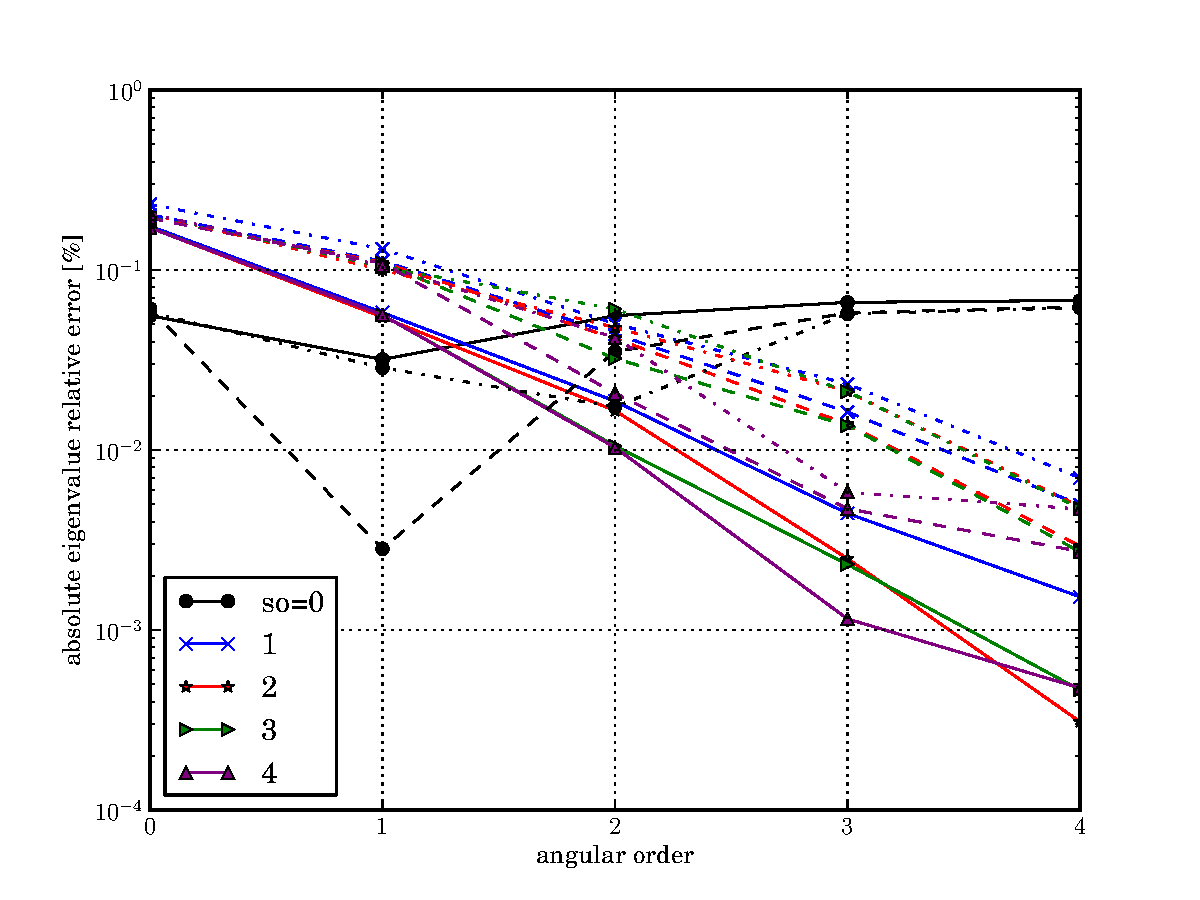
\includegraphics[keepaspectratio, width = 5.0 in]
                    {takeda_order_study_eigenvalue_error}
    \caption{Takeda problem absolute relative eigenvalue error as 
             a function of angular order for several spatial orders.  
             The solid lines indicate the conservative basis, while the 
             dashed and dashed-dot lines indicate the DLP basis used to 
             expand the angular flux $\psi$ and current $J$, respectively.}
    \label{fig:takeda_order_study_eigenvalue_error}
\end{figure}

\begin{figure}[ht]
    \centering
    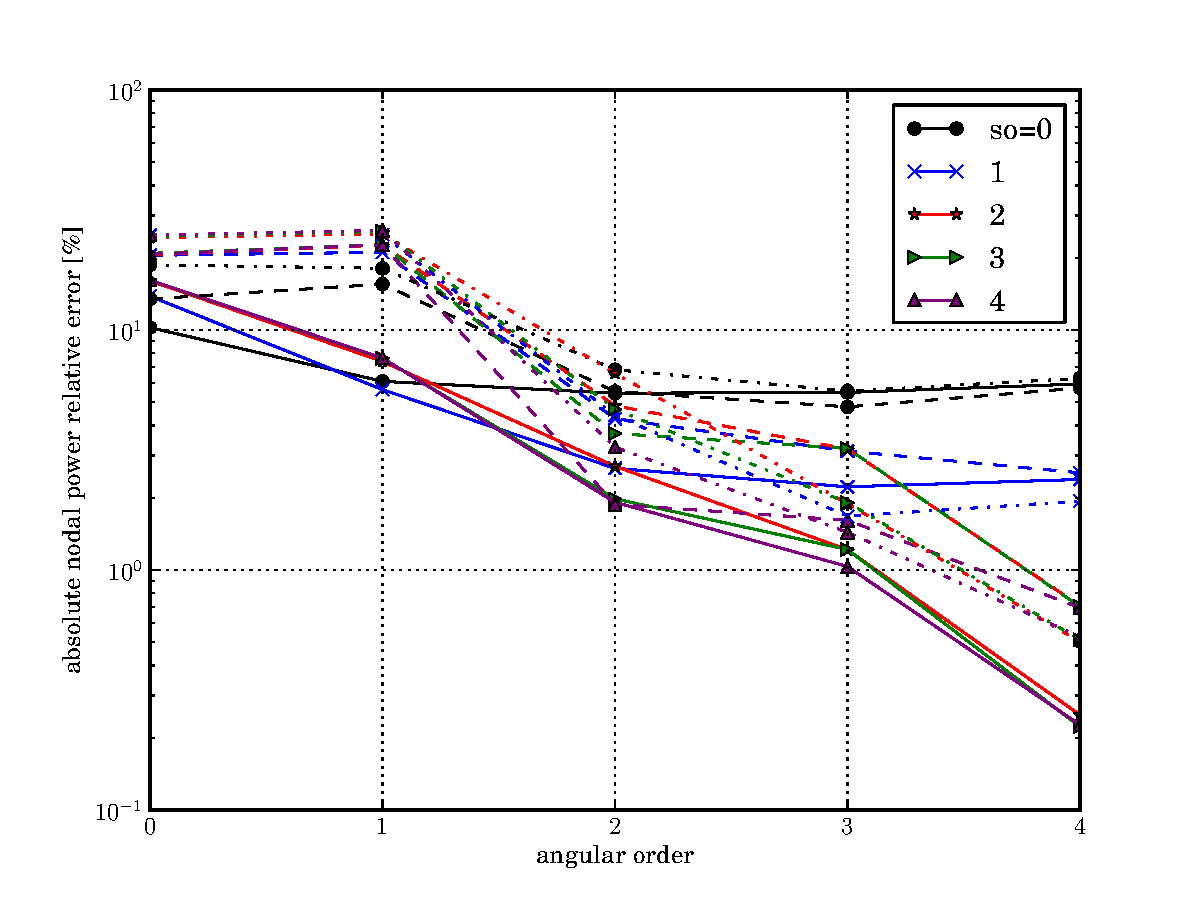
\includegraphics[keepaspectratio, width = 5.0 in]
                    {takeda_order_study_nodal_power_error}
    \caption{Takeda problem absolute relative nodal power error as 
             a function of angular order for several spatial orders.  
             The solid lines indicate the conservative basis, while the 
             dashed and dashed-dot lines indicate the DLP basis used to 
             expand the angular flux $\psi$ and current $J$, respectively.}
    \label{fig:takeda_order_study_nodal_power_error}
\end{figure}

\subsubsection{Solver Comparison}

The same set of solvers as used for the diffusion problems 
and the 2-D C5G7 problem were applied to a the Takeda problem. A second 
order spatial expansion with a third order angular expansion in the 
azimuth and polar variables was used.  Order reduction was applied to both 
the spatial and angular terms.  The problem was run on 64 processors, with 
one process for the global problem.  Table \ref{tbl:takeda_outer_study} 
provides the wall time, total time summed over all processors, and the 
total response function time summed over all processors.  

Similar to the diffusion results, the extrapolated Picard iteration 
proves to be the most efficient of the solvers studied.  
Newton's method with the coarse $k$ finite difference yielded just as 
few $k$-evaluations but with a slightly higher overall cost.

\begin{table}[ht] 
 \begin{center} 
 
  \begin{threeparttable}
 \begin{tabular}{ccccccc} 
 \toprule 
  solver & w. time\tnote{f} [s]& time\tnote{g} [s] & r. time\tnote{h} [s] & inners & outers & $k$-evals. \\
  \midrule
    P\tnote{a}            &  $9.76\cdot 10^2$ &  $6.25\cdot 10^4$ &  $5.91\cdot 10^4$ &           56 &           13 &           14 \\ 
    P+exp\tnote{b}       &  $3.51\cdot 10^2$ &  $2.24\cdot 10^4$ &  $2.12\cdot 10^4$ &           23 &        4 &   5  \\ 
    S\tnote{c}            &  $1.05\cdot 10^3$ &  $6.72\cdot 10^4$ &  $6.36\cdot 10^4$ &           58 &            7 &           15 \\ 
    N+$\delta k$\tnote{d}&  $7.30\cdot 10^2$ &  $4.67\cdot 10^4$ &  $4.26\cdot 10^4$ &           57 &            5 &           10 \\ 
    N+$\Delta k$\tnote{e}&  $3.87\cdot 10^2$ &  $2.48\cdot 10^4$ &  $2.14\cdot 10^4$ &           44 &          4 &           5  \\ 
 \bottomrule 
 \end{tabular} 
 
 
 {\footnotesize
 \begin{tablenotes}
   \item[a] Picard 
   \item[b] Picard with exponential extrapolation
   \item[c] Steffensen
   \item[d] Newton with fine $k$ difference
   \item[e] Newton with coarse $k$ difference
   \item[f] Wall time
   \item[g] Total time summed over all processes
   \item[h] Total response generation time summed over all processes
 \end{tablenotes}
 }
 
 \end{threeparttable}
 
 \end{center} 
 \caption{Outer solver comparison for 3-D Takeda problem with second order 
          spatial expansion and third order polar and azimuthal angle 
          expansions.} 
 \label{tbl:takeda_outer_study} 
\end{table} 

\subsection{Summary}

Based on the results for both the diffusion and transport problems, Picard 
iteration with the exponential extrapolation appears generally to be the most
efficient of the methods, yielding minimum numbers of $k$-evaluations 
while providing the lowest global solver overhead.  However, the 
extrapolation is based on $\lambda$ converging to unity, and because this 
is not always guaranteed, Newton's method with the coarse finite difference 
provides a more consistently robust solver, with nearly as 
few $k$-evaluations and only relatively small overhead due to the 
inner linear solves.

It is anticipated further work on preconditioners for Newton's method 
would put the corresponding (global) computation time more in line with 
that of the extrapolated Picard iteration.  Even so, the efficacy and 
simplicity of the Picard iteration suggests that care should be taken to 
select a conservative basis leading to $\lambda = 1$ upon convergence.

